\documentclass[12pt]{article}
\usepackage{graphicx} % Required for inserting images
\usepackage[utf8]{inputenc}
\usepackage[T1]{fontenc}  % Wichtig für Trennung von Wörtern
\usepackage{csquotes}
\usepackage{bbm}
\usepackage{amsmath}
\usepackage{amssymb}
\usepackage{amsthm}
\usepackage{mathtools}
\usepackage{url}
\usepackage{enumitem}
\usepackage[
colorlinks=true, 
linkcolor=blue,
citecolor=blue,
urlcolor=blue
]{hyperref}
\usepackage{cleveref}
\usepackage{setspace}
\usepackage{tikz}
\usetikzlibrary{positioning}

\usepackage[style=numeric]{biblatex}
\addbibresource{literatur.bib}

\onehalfspacing
\allowdisplaybreaks

\newcommand{\N}{\mathbbm{N}} % natürliche Zahlen
\newcommand{\Z}{\mathbbm{Z}} % ganze Zahlen
\newcommand{\R}{\mathbb{R}} % reelle Zahlen
\newcommand{\C}{\mathbb{C}} % komplexe Zahlen
\newcommand{\Q}{\mathbb{Q}} % rationale Zahlen

\newtheorem{satz}{Satz}[section]
\newtheorem{definition}[satz]{Definition}
\newtheorem{lemma}[satz]{Lemma}
\newtheorem{beispiel}[satz]{Beispiel}
\newtheorem{algorithmus}[satz]{Algorithmus}
\newtheorem{korollar}[satz]{Korollar}

\title{
Einfache Graphenalgorithmen\\[0.5em]
\Large Ausarbeitung zum Vortrag\\
Proseminar Kombinatorik\\
Sommersemester 2026
}

\author{
Lennart Meier\\
\url{lennart.meier05@gmail.com}
}

\date{26.05.2026}

\begin{document}

\maketitle
\thispagestyle{empty}

\newpage

\pagenumbering{roman}

\tableofcontents

\newpage

\pagenumbering{arabic}

\section{Einleitung}

Diese Ausarbeitung behandelt einfache Graphenalgorithmen und basiert auf Kapitel 7 aus \cite{hougardy2018}. 
Graphen gehören zu den wichtigsten Strukturen der Mathematik und Informatik. Viele Probleme lassen sich mithilfe von Graphen darstellen. Beispiele hierfür sind:

\begin{itemize}
    \item Straßennetze, Bahnnetze,
    \item soziale Netzwerke,
    \item Kommunikationsnetze,
    \item Projektplanung.
\end{itemize}

Ein zentrales Problem besteht darin, einen Graphen systematisch zu durchsuchen und Informationen über seine Struktur zu gewinnen. Dabei interessiert insbesondere:

\begin{itemize}
    \item welche Knoten erreichbar sind
    \item wie kürzeste Wege bestimmt werden können
    \item ob ein Graph bipartit ist
    \item ob ein gerichteter Graph Kreise enthält
\end{itemize}
Im Folgenden werden zunächst allgemeine Verfahren zur Graphendurchmusterung vorgestellt. Anschließend werden spezielle Algorithmen wie Tiefensuche und Breitensuche untersucht. Danach werden bipartite Graphen sowie azyklische Digraphen betrachtet.

\section{Grundbegriffe/Wiederholung Graphen}

\begin{definition}
Ein Graph ist ein Paar
\[
G=(V,E),
\]
wobei
\begin{itemize}
    \item \(V\) eine endliche Menge von Knoten ist,
    \item \(E\) eine Menge von Kanten ist.
\end{itemize}
\end{definition}

Bei ungerichteten Graphen besteht jede Kante aus einer ungeordneten Menge
\[
\{u,v\}.
\]

Bei gerichteten Graphen besitzen die Kanten dagegen eine Richtung und werden als geordnete Paare
\[
(u,v)
\]
geschrieben.

\begin{beispiel}
Der folgende Graph besitzt vier Knoten und vier Kanten:

\begin{center}
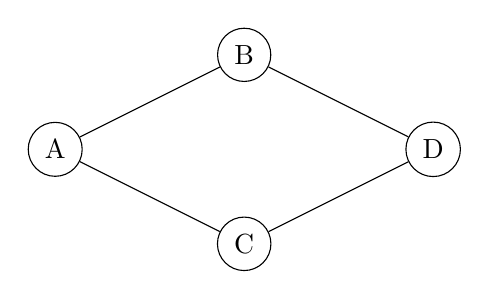
\begin{tikzpicture}[scale=1.2]

\node[circle,draw] (A) at (0,0) {A};
\node[circle,draw] (B) at (2,1) {B};
\node[circle,draw] (C) at (2,-1) {C};
\node[circle,draw] (D) at (4,0) {D};

\draw (A)--(B);
\draw (A)--(C);
\draw (B)--(D);
\draw (C)--(D);

\end{tikzpicture}
\end{center}

Es gilt:
\[
V=\{A,B,C,D\},
\]
\[
E=\{\{A,B\},\{A,C\},\{B,D\},\{C,D\}\}.
\]
\end{beispiel}

\begin{definition}
Ein Weg ist eine Folge von Knoten, bei der aufeinanderfolgende Knoten durch eine Kante verbunden sind.

Ein Kreis ist ein geschlossener Weg.

Ein Graph heißt zusammenhängend, wenn zwischen je zwei Knoten ein Weg existiert.
\end{definition}

\section{Graphendurchmusterung}

Das grundlegende Verfahren zur Untersuchung eines Graphen ist die sogenannte Graphendurchmusterung.

\begin{algorithmus}[Graphendurchmusterung]

Eingabe: ein Graph \(G\), ein Knoten \(r \in V(G)\)

Ausgabe: die Menge \(R \subseteq V(G)\) der von \(r\) aus erreichbaren Knoten und eine Menge \(F \subseteq E(G)\), sodass \((R,F)\) ein Baum beziehungsweise eine Arboreszenz mit Wurzel \(r\) ist.

\begin{align*}
&R \leftarrow \{r\},\quad Q \leftarrow \{r\},\quad F \leftarrow \emptyset\\
&\textbf{while } Q \neq \emptyset \textbf{ do}\\
&\qquad \text{Wähle ein } v \in Q\\
&\qquad \textbf{if } \exists e=(v,w)\in \delta_G^+(v)\\
&\qquad\qquad \text{mit } w\in V(G)\setminus R\\
&\qquad \textbf{then } R\leftarrow R\cup\{w\}\\
&\qquad\qquad Q\leftarrow Q\cup\{w\}\\
&\qquad\qquad F\leftarrow F\cup\{e\}\\
&\qquad \textbf{else } Q\leftarrow Q\setminus\{v\}
\end{align*}
\end{algorithmus}

\newpage 

\begin{satz}
Der Algorithmus zur Graphendurchmusterung arbeitet korrekt und kann mit Laufzeit
\[
O(n+m)
\]
implementiert werden, wobei
\[
n=|V(G)|,\qquad m=|E(G)|.
\]
\end{satz}

\begin{proof}
Zu Beginn besteht \((R,F)\) lediglich aus dem Startknoten \(r\). Somit ist \((R,F)\) ein Baum beziehungsweise eine Arboreszenz mit Wurzel \(r\).

Im Verlauf des Algorithmus wird genau ein neuer Knoten \(w\) zusammen mit einer Kante \(e\) hinzugefügt, wobei der andere Endknoten der Kante bereits in \(R\) liegt. Dadurch bleibt die Baumstruktur erhalten.
Angenommen, am Ende des Algorithmus gäbe es einen von \(r\) aus erreichbaren Knoten \(w\), der nicht in \(R\) enthalten ist. Dann existiert ein Weg von \(r\) nach \(w\). Auf diesem Weg muss es eine Kante geben, die einen Knoten aus \(R\) mit einem Knoten außerhalb von \(R\) verbindet. Eine solche Kante hätte der Algorithmus jedoch betrachtet und den neuen Knoten hinzugefügt. Dies ist ein Widerspruch.
Für die Laufzeit betrachtet man jede Kante höchstens zweimal. Jeder Knoten wird höchstens einmal eingefügt und entfernt. Daher ergibt sich insgesamt eine lineare Laufzeit
\[
O(n+m).
\]
\end{proof}

\begin{korollar}
Die Zusammenhangskomponenten eines ungerichteten Graphen können in linearer Zeit bestimmt werden.
\end{korollar}

\begin{proof}
Man startet den Algorithmus in einem beliebigen Knoten. Falls nicht alle Knoten erreicht werden, bildet die Menge der erreichten Knoten eine Zusammenhangskomponente. Anschließend wiederholt man den Algorithmus auf den verbleibenden Knoten.
\end{proof}

\section{Tiefensuche}

Eine wichtige Variante der Graphendurchmusterung ist die Tiefensuche.

\begin{definition}
Wählt man in der Menge \(Q\) stets den zuletzt hinzugefügten Knoten aus, so erhält man die Tiefensuche beziehungsweise DFS (\emph{Depth First Search}).
\end{definition}

Die Tiefensuche arbeitet nach dem Prinzip:
\begin{quote}
Gehe erst möglichst tief in den Graphen, bevor man zurück geht.
\end{quote}

Dafür verwendet DFS einen Stack.

\begin{beispiel}
Eine mögliche DFS-Reihenfolge im folgenden Graphen lautet:
\[
A,B,D,C,E.
\]

\begin{center}
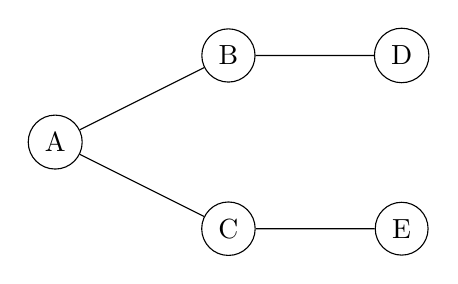
\begin{tikzpicture}[scale=1.1]

\node[circle,draw] (A) at (0,0) {A};
\node[circle,draw] (B) at (2,1) {B};
\node[circle,draw] (C) at (2,-1) {C};
\node[circle,draw] (D) at (4,1) {D};
\node[circle,draw] (E) at (4,-1) {E};

\draw (A)--(B);
\draw (A)--(C);
\draw (B)--(D);
\draw (C)--(E);

\end{tikzpicture}
\end{center}
\end{beispiel}

DFS wird unter anderem verwendet für:
\begin{itemize}
    \item Zusammenhangsprobleme,
    \item Kreissuche,
    \item topologische Sortierung,
    \item Komponentenzerlegungen.
\end{itemize}

\section{Breitensuche}

\begin{definition}
Wählt man in der Menge \(Q\) stets den zuerst hinzugefügten Knoten aus, so erhält man die Breitensuche beziehungsweise BFS (\emph{Breadth First Search}).
\end{definition}

BFS durchsucht den Graphen schichtweise. Zunächst werden alle Nachbarn des Startknotens besucht, danach alle Nachbarn dieser Knoten usw.

Hierfür wird eine Queue verwendet.

\begin{beispiel}
Im folgenden Graphen ergeben sich die BFS-Ebenen
\[
\{A\},\{B,C,D\},\{E,F\}.
\]

\begin{center}
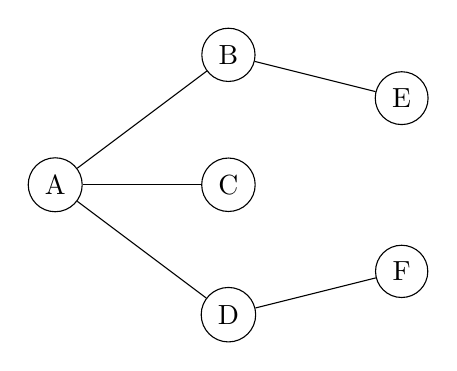
\begin{tikzpicture}[scale=1.1]

\node[circle,draw] (A) at (0,0) {A};

\node[circle,draw] (B) at (2,1.5) {B};
\node[circle,draw] (C) at (2,0) {C};
\node[circle,draw] (D) at (2,-1.5) {D};

\node[circle,draw] (E) at (4,1) {E};
\node[circle,draw] (F) at (4,-1) {F};

\draw (A)--(B);
\draw (A)--(C);
\draw (A)--(D);
\draw (B)--(E);
\draw (D)--(F);

\end{tikzpicture}
\end{center}
\end{beispiel}

Für zwei Knoten \(v,w\) bezeichnet
\[
dist(v,w)
\]
die Länge eines kürzesten Weges von \(v\) nach \(w\).

\begin{satz}
Jeder BFS-Baum enthält einen kürzesten Weg von einem Knoten \(r\) zu allen anderen von \(r\) aus erreichbaren Knoten.
\end{satz}

\begin{proof}
Die Breitensuche arbeitet schichtweise. Zunächst werden alle Knoten mit Abstand \(1\) besucht, danach alle Knoten mit Abstand \(2\) usw.

Ein Knoten wird also erstmals genau dann erreicht, wenn ein kürzester Weg zu ihm gefunden wurde. Daher enthält der BFS-Baum nur kürzeste Wege.
\end{proof}

\begin{satz}
Die Werte
\[
dist(r,v)
\]
können für alle Knoten \(v\) in linearer Zeit bestimmt werden.
\end{satz}

\begin{proof}
Jeder Knoten wird höchstens einmal besucht und jede Kante höchstens zweimal betrachtet. Daher beträgt die Laufzeit insgesamt
\[
O(n+m).
\]
\end{proof}

\section{Bipartite Graphen}

\begin{definition}
Eine Bipartition eines ungerichteten Graphen \(G\) besteht aus zwei disjunkten Knotenmengen \(A\) und \(B\), deren Vereinigung \(V(G)\) ist, sodass jede Kante genau einen Endknoten in \(A\) besitzt.
Ein Graph heißt bipartit, falls er eine Bipartition besitzt.
\end{definition}

\begin{definition}
Ein ungerader Kreis ist ein Kreis ungerader Länge.
\end{definition}

\begin{satz}[König]
Ein ungerichteter Graph ist genau dann bipartit, wenn er keinen ungeraden Kreis enthält.
\end{satz}

\begin{proof}
Sei zunächst \(G\) bipartit mit Bipartition
\[
V(G)=A\cup B.
\]

Durchläuft man einen Kreis, so wechselt man nach jeder Kante zwischen den Mengen \(A\) und \(B\). Daher muss jeder Kreis gerade Länge besitzen. Somit existiert kein ungerader Kreis.
Nun sei umgekehrt \(G\) ein Graph ohne ungeraden Kreis. Man führt eine Breitensuche mit Startknoten \(r\) durch und definiert:
\[
A:=\{v\in V(G)\mid dist(r,v)\text{ gerade}\},
\]
\[
B:=V(G)\setminus A.
\]
Angenommen, es gäbe eine Kante innerhalb einer der beiden Mengen. Dann entstünde zusammen mit den BFS-Wegen ein ungerader Kreis. Dies widerspricht der Voraussetzung.
Folglich ist der Graph bipartit.
\end{proof}

\section{Azyklische Digraphen}

\begin{definition}
Ein Digraph heißt azyklisch, falls er keinen gerichteten Kreis enthält.
\end{definition}

\begin{definition}
Sei
\[
V(G)=\{v_1,\dots,v_n\}.
\]

Eine topologische Ordnung ist eine Ordnung der Knoten, sodass
\[
i<j
\]
für jede Kante
\[
(v_i,v_j)\in E(G)
\]
gilt.
\end{definition}

\begin{lemma}
Ist \(G\) ein Digraph mit
\[
\delta^+(v)\neq \emptyset
\]
für alle \(v\in V(G)\), so kann man in
\[
O(|V(G)|)
\]
Zeit einen Kreis in \(G\) finden.
\end{lemma}

\begin{proof}
Man startet in einem beliebigen Knoten und folgt jeweils einer ausgehenden Kante. Da der Graph nur endlich viele Knoten besitzt, muss irgendwann ein Knoten erneut besucht werden. Dadurch entsteht ein Kreis.
\end{proof}

\begin{satz}
Ein Digraph besitzt genau dann eine topologische Ordnung, wenn er azyklisch ist.
\end{satz}

\begin{proof}
Besitzt ein Digraph eine topologische Ordnung, so kann kein gerichteter Kreis existieren, da entlang jeder Kante die Nummerierung streng anwächst. Nun sei \(G\) azyklisch. Dann existiert mindestens ein Knoten ohne ausgehende Kante. Entfernt man diesen Knoten, bleibt erneut ein azyklischer Graph zurück. Durch wiederholtes Entfernen solcher Knoten entsteht schließlich eine Reihenfolge
\[
v_1,\dots,v_n,
\]
die eine topologische Ordnung bildet.
\end{proof}

\section{Fazit}

In dieser Ausarbeitung wurden einfache Graphenalgorithmen untersucht. Die Graphendurchmusterung bildet die Grundlage vieler weiterer Verfahren. Besonders wichtig sind die beiden Varianten Tiefensuche und Breitensuche. Die Breitensuche ermöglicht zusätzlich die Berechnung kürzester Wege in ungewichteten Graphen. Außerdem liefert sie wichtige Anwendungen beim Test auf Bipartitheit. Außerdem wurden azyklische Digraphen betrachtet. Für diese Graphen existieren topologische Ordnungen, die insbesondere bei Abhängigkeitsproblemen verwendet werden.

\newpage
\printbibliography[heading=bibintoc]

\end{document}
